\documentclass[11pt,a4paper,oneside]{article}
\usepackage[latin1]{inputenc}
\usepackage{amsmath}
\usepackage{amsfonts}
\usepackage{amssymb}
\usepackage{graphicx}
\usepackage{color}
\usepackage {tikz}
\usetikzlibrary {er}
\usepackage[left=2.00cm, right=2.00cm, top=1.00cm]{geometry}
\graphicspath{{./}}

\begin{document}
	\title{DS 221 - Introduction to Scalable Systems \\ Assignment 2}
	\author{Shriram R. \\ M Tech (CDS) \\ 06-02-01-10-51-18-1-15763}
	\maketitle
	
	\section{2D Matrices}
	The 2D matrix abstract data structure has been implemented using 2D array and compressed sparse matrix representation (CSR) and the space and time complexities has been analyzed and empirically verified.
	The following sections will cover the analysis and empirical results in detail.
	
	\subsection{Storage Space}
	Let N, M and NNZ denote the number of rows, columns and non-zero elements of the matrix respectively. This notation is adopted for the remainder of this report. For 2D array implementation, space gets allocated to each element irrespective of its value and so the asymptotic space complexity is O(NM) (independent of NNZ). \\
	\newline
	For CSR implementation, we have three 1D arrays namely A for storing matrix values, IA for storing the cumulative number of non-zero values for each row and JA for storing the column index for each non-zero value. These arrays have NNZ, N+1 and NNZ elements respectively. Hence, the asymptotic space complexity is O(N + 2NNZ). In the worst case where NNZ = NM (all elements are non zero), CSR will take more space as its space complexity goes to O(N + 2NM). \\
	\newline
	The space complexities has been empirically determined for different matrix sizes and the results plotted below match with the analysis. Square matrices (N=M) were used for simplicity of analysis.
	
	\begin{center}
		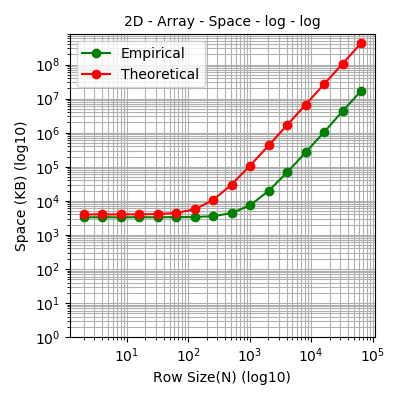
\includegraphics[scale=0.6]{1.png}		
	\end{center}

	\begin{center}
		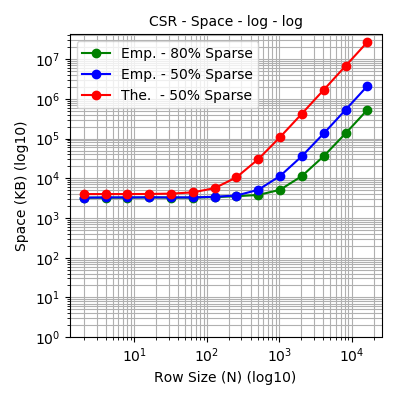
\includegraphics[scale=0.6]{2.png}		
	\end{center}

    For CSR, the sparse percentage denotes the percentage of elements that are zero in the matrix.

    \subsection{Matrix Addition}
    For matrix addition, all the elements of both input and output matrices have to be processed exactly once and there are NM elements in each matrix. In the case of 2D array implementation, each element can be accessed in O(1) time and so the total time complexity for addition in this case is O(NM). Note that the effects of locality and caching is ignored in this analysis. \\
    \newline
    For the case of CSR implementation, each element can be accessed in O(M) time assuming the worst case where all the elements are non-zero. This is because the array JA has to be scanned for matching column index in order to access an element. So, the worst case time complexity for addition in this case will be $O(NM^2)$. \\   
    \newline
    The time complexities has been empirically determined for different matrix sizes and the results plotted below match with the analysis. Square matrices (N=M) were used for simplicity of analysis,
    
    \begin{center}
    	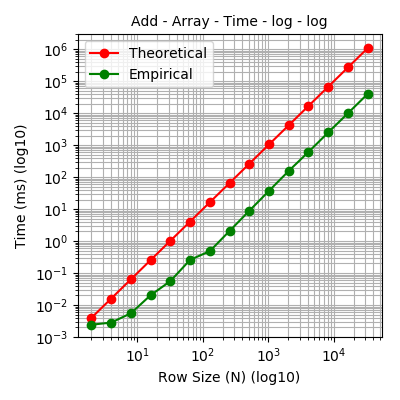
\includegraphics[scale=0.6]{3.png}		
    \end{center}
    
    \begin{center}
    	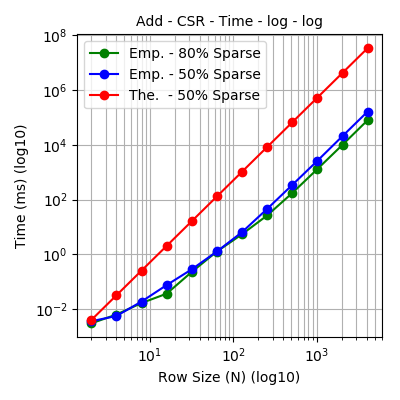
\includegraphics[scale=0.6]{4.png}		
    \end{center}
    
    \subsection{Matrix Multiplication}
    For matrix multiplication, analysis is done for multiplying two NxN square matrices without loss of generality. The naive or brute force implementation of the algorithm takes $O(N^3)$ multiplication and addition operations. Similar to addition, cache and locality effects are ignored in the analysis. \\
    \newline
    In the case of 2D array implementation, each element can be accessed in $O(1)$ time and so the total time complexity for multiplication in this case is $O(N^3)$. \\
    \newline
    For the case of CSR implementation, each element can be accessed in $O(N)$ time assuming the worst case where all the elements are non-zero. So, the time complexity for multiplication in this case will be $O(N^4)$. \\   
    \newline    
    The time complexities has been empirically determined for different matrix sizes and the results plotted below match with the analysis,
    
     \begin{center}
    	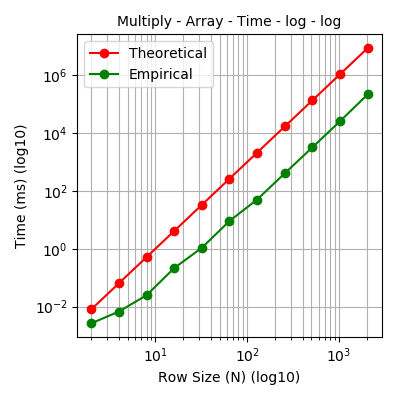
\includegraphics[scale=0.6]{5.png}		
    \end{center}
    
    \begin{center}
    	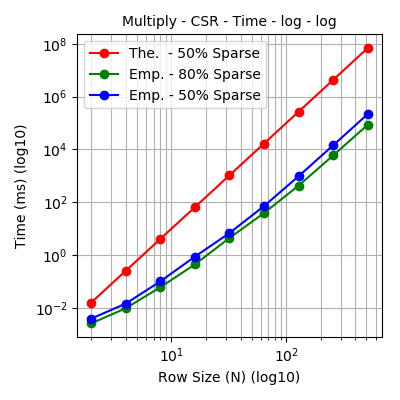
\includegraphics[scale=0.6]{6.png}		
    \end{center}

    \subsection{Breadth First Search}
    
    Let V be the number of nodes and E be the number of edges. The breadth first search algorithm has the following components,
    \begin{list}{*}{}
    	\item Inserting and removing nodes from the queue. Each node will be inserted and removed once. So, the time complexity for this component is O(V)
    	\item Scanning the neighbors for each node once. The current CSR implementation will take O(V) (Max. degree) time to check if a node is a neighbor in the worst case. So, the time complexity is $O(V^3)$ for performing scan of neighbors for all the nodes
    	\item Inserting the visited nodes to the STL list. The time complexity is O(V)
    	\item Sorting the list of nodes in each depth. The time complexity is O(V log V) 
    \end{list}
    It can be inferred that the total time complexity is $O(V^3)$.

    \begin{center}
    	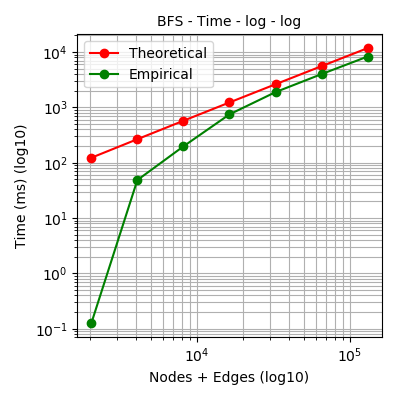
\includegraphics[scale=0.6]{7.png}		
    \end{center}

    \section{Code and Testing Remarks}
    The makefile has been modified to use the C++ 11 standard during compilation. This is because the code uses some string parsing functions like std::stoi, std::stof etc. which are not available as part of C++ 98 standard. \\
    \newline
    The precision of the output is set by std::fixed and std::setprecision functions. The memory used by the program has been measured using the \emph{time} shell program and the time is measured using clock\_gettime() function. \\
    \newline
    Input files with random float numbers were generated for the purpose of empirical testing. The tests were run using custom shell scripts. [4] is the location of these scripts in the cluster.
    
    \section{References}
    
    \begin{list}{}{}
    	\item 1. https://en.cppreference.com/
    	\item 2. https://www.geeksforgeeks.org/
    	\item 3. DS 221 Course lecture notes
    	\item 4. /home/shriramr/ds221/part\_2/code/test
    \end{list}

\end{document}